% vim: set tw=78 tabstop=4 shiftwidth=4 aw ai:
\documentclass{beamer}

\usepackage[utf8x]{inputenc}		% diacritice
\usepackage[english]{babel}
\usepackage{color}			% highlight
\usepackage{alltt}			% highlight

\usepackage{hyperref}			% folosiți \url{http://...}
					% sau \href{http://...}{Nume Link}
\usepackage{verbatim}

\mode<presentation>
{ \usetheme{Berlin} }

% Încărcăm simbolurilor Unicode românești în titlu și primele pagini
\PreloadUnicodePage{200}

% Arătăm numărul frame-ului
\newcommand{\frameofframes}{/}
\newcommand{\setframeofframes}[1]{\renewcommand{\frameofframes}{#1}}

\setframeofframes{of}
\makeatletter
\setbeamertemplate{footline}
  {%
    \begin{beamercolorbox}[colsep=1.5pt]{upper separation line foot}
    \end{beamercolorbox}
    \begin{beamercolorbox}[ht=2.5ex,dp=1.125ex,%
      leftskip=.3cm,rightskip=.3cm plus1fil]{author in head/foot}%
      \leavevmode{\usebeamerfont{author in head/foot}\insertshortauthor}%
      \hfill%
      {\usebeamerfont{institute in head/foot}\usebeamercolor[fg]{institute in head/foot}\insertshortinstitute}%
    \end{beamercolorbox}%
    \begin{beamercolorbox}[ht=2.5ex,dp=1.125ex,%
      leftskip=.3cm,rightskip=.3cm plus1fil]{title in head/foot}%
      {\usebeamerfont{title in head/foot}\insertshorttitle}%
      \hfill%
      {\usebeamerfont{frame number}\usebeamercolor[fg]{frame number}\insertframenumber~\frameofframes~\inserttotalframenumber}
    \end{beamercolorbox}%
    \begin{beamercolorbox}[colsep=1.5pt]{lower separation line foot}
    \end{beamercolorbox}
  }
\makeatother

\setbeamertemplate{navigation symbols}{}%remove navigation symbols

\title[Multipath TCP Ninja Tunneling on Mobile Devices]{Multipath TCP Ninja Tunneling on Mobile Devices}
\subtitle{Master Report Session -- June 2015}
\institute{Faculty of Automatic Control and Computers,\\
	University POLITEHNICA of Bucharest}
\author[Silviu Petria, Silviu-Mihai Popescu]{Silviu Petria, Silviu-Mihai
Popescu\\
	Supervisor: Costin Raiciu}
\date{June 12, 2015}

\begin{document}

% Slide-urile cu mai multe părți sunt marcate cu textul (cont.)
\setbeamertemplate{frametitle continuation}[from second]

\frame{\titlepage}

\section{Ninja Tunneling}
\begin{frame}{Ninja Tunneling}
  \begin{itemize}
    \item Multiple OpenVPN tunnels on common ports
    \item MPTCP using all tunnels
     \item Use cases
    \begin{itemize}
      \item bypassing egress firewalls
      \item avoiding middlebox interference
      \item avoiding cellular operators restrictions
    \end{itemize}
  \end{itemize}
\end{frame}

\section{Cellular Operators Analysis}
\begin{frame}{Romanian Cellular Operators Analysis}
\begin{center}
    \begin{table}
    \centering
    \begin{tabular}{ | l | l | l | l | }
    \hline
    Name & Filters MPTCP & Port shaping & Application shaping \\ \hline
    Operator 1 & Yes & Yes & Yes  \\ \hline
    Operator 2 & Yes & Yes & No \\ \hline
    Operator 3 & No & Yes & No \\ \hline
    Operator 4 & Yes & Yes & No \\ \hline
    \end{tabular}
    \label{table:operators}
    \end{table}
\end{center}
\end{frame}

\section{Setup}
\begin{frame}{Setup}
   \begin{itemize}
	\item Galaxy Nexus phone running a custom MPTCP kernel
           \item Public-IP Linux machine serving as endpoint for OpenVPN tunnels
           \item Tunnels
	\begin{itemize}
		\item UDP 1194
		\item TCP 1195
		\item TCP 80
		\item UDP 53
	\end{itemize}
    	\item Testing download and upload using CUBIC and OLIA
    \end{itemize}
\end{frame}

\section{CUBIC}
\begin{frame}{CUBIC Upload}
  \begin{figure}
    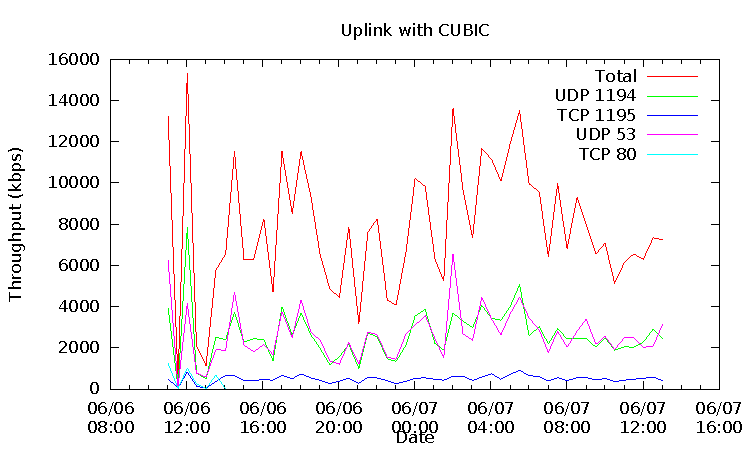
\includegraphics[scale=0.75]{img/up-cubic}
  \end{figure}
\end{frame}
\begin{frame}{CUBIC Download}
  \begin{figure}
    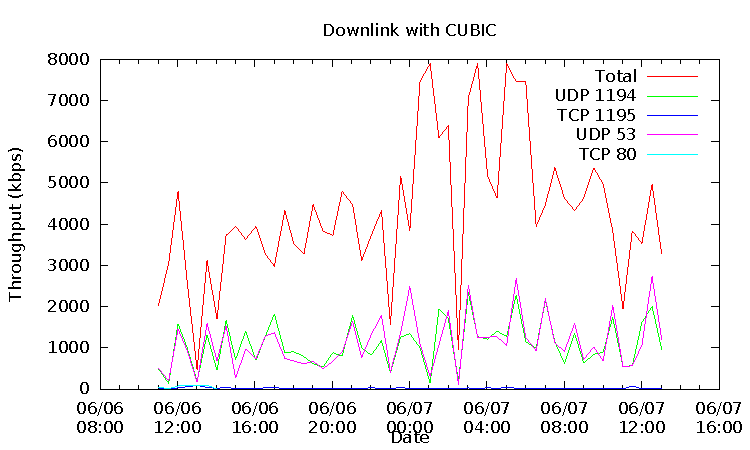
\includegraphics[scale=0.75]{img/down-cubic}
  \end{figure}
\end{frame}

\section{OLIA}
\begin{frame}{OLIA Upload}
  \begin{figure}
    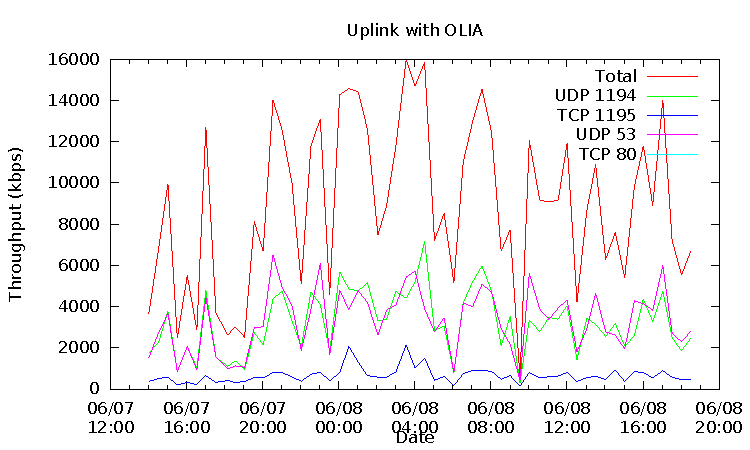
\includegraphics[scale=0.75]{img/up-olia}
  \end{figure}
\end{frame}
\begin{frame}{OLIA Download}
  \begin{figure}
    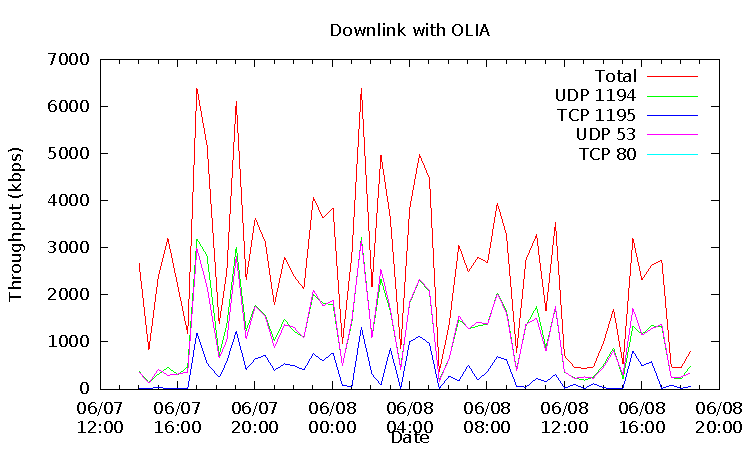
\includegraphics[scale=0.75]{img/down-olia}
  \end{figure}
\end{frame}

\section{Throughput distribution}
\begin{frame}{Throughput Distribution}
\begin{center}
	\begin{table}[htb]
	\centering
	\begin{tabular}{ | l | l | l | l | l | }
	\hline
	& UDP (1194) & TCP (1195) & DNS (53) & HTTP (80) \\ \hline
	CUBIC & 45.75\% & 8.88\% &  45.37\% & 0\%\footnote{During the small time frame it was active, the HTTP tunnel contributed roughly 1\% of the throughput and the contribution of the TCP tunnel was slightly reduced.} \\ \hline
	OLIA & 46.77\% & 7.74\% & 45.49\% & 0\% \\ \hline
	\end{tabular}
	\label{table:iodine}
	\end{table}
\end{center}
\end{frame}

\section{Iodine}
\begin{frame}{Iodine}
	\begin{itemize}
		\item IP-over-DNS solution
		\item places data inside DNS queries
	\end{itemize}
	\begin{center}
	\begin{table}[htb]
	\centering
	\resizebox{\textwidth}{!}{\begin{tabular}{ | l | l | l | l | l | }
	\hline
	& TCP up (Mbps) & UDP up (Mbps) & UDP loss (\%) & HTTP down (Mbps) \\ \hline
	Baseline & 1.15 & 1.39 &  0.11 & 2.5 \\ \hline
	Iodine & 1.14 & 1.32 & 2.6 & 2.35 \\ \hline
	OpenVPN & 0.087 & 0.55 & 49 & N/A \\ \hline
	\end{tabular}}
	\caption{Throughput comparison between Iodine, OpenVPN and default 3G. Average of ten tests run during daytime hours.}
	\label{table:iodine}
	\end{table}
	\end{center}
\end{frame}

\section{Conclusion}
\begin{frame}{Conclusion}
	\begin{itemize}
	\item Throughput achieved on par with normal communication
	\item Added benefit of encryption and multiple paths
	\item Circumventing operator restrictions
	\item Shedding light on how operators perform traffic shaping
	\end{itemize}
\end{frame}
\end{document}
